%%%%%%%%%%%%%%%%%%%%%%%%%%%%%%%%%%%%%%%%%%%%%%%%%%%%%%%%%%%%%%%%%%%%%%%%%%%%%%%%
%% Plantilla de memoria en LaTeX para la ETSIT - Universidad Rey Juan Carlos
%%
%% Por Gregorio Robles <grex arroba gsyc.urjc.es>
%%     Grupo de Sistemas y Comunicaciones
%%     Escuela Técnica Superior de Ingenieros de Telecomunicación
%%     Universidad Rey Juan Carlos
%% (muchas ideas tomadas de Internet, colegas del GSyC, antiguos alumnos...
%%  etc. Muchas gracias a todos)
%%
%% La última versión de esta plantilla está siempre disponible en:
%%     https://github.com/gregoriorobles/plantilla-memoria
%%
%% Para obtener PDF, ejecuta en la shell:
%%   make
%% (las imágenes deben ir en PNG o JPG)

%%%%%%%%%%%%%%%%%%%%%%%%%%%%%%%%%%%%%%%%%%%%%%%%%%%%%%%%%%%%%%%%%%%%%%%%%%%%%%%%

\documentclass[a4paper, 17pt]{book}
%\usepackage[T1]{fontenc}

\usepackage[a4paper, left=2.5cm, right=2.5cm, top=3cm, bottom=3cm]{geometry}
\usepackage{times}
\usepackage[utf8]{inputenc}
\usepackage[spanish]{babel} % Comenta esta línea si tu memoria es en inglés
\usepackage{url}
%\usepackage[dvipdfm]{graphicx}
\usepackage{graphicx}
\usepackage{float}  %% H para posicionar figuras
\usepackage[nottoc, notlot, notlof, notindex]{tocbibind} %% Opciones de índice
\usepackage{latexsym}  %% Logo LaTeX

\title{Memoria del Proyecto}
\author{Nombre del autor}

\renewcommand{\baselinestretch}{1.5}  %% Interlineado

\begin{document}

\renewcommand{\refname}{Bibliografía}  %% Renombrando
\renewcommand{\appendixname}{Apéndice}

%%%%%%%%%%%%%%%%%%%%%%%%%%%%%%%%%%%%%%%%%%%%%%%%%%%%%%%%%%%%%%%%%%%%%%%%%%%%%%%%
% PORTADA

\begin{titlepage}
\begin{center}
\begin{tabular}[c]{c c}
%\includegraphics[bb=0 0 194 352, scale=0.25]{logo} &
\includegraphics[scale=0.25]{img/logo_vect.png} &
\begin{tabular}[b]{l}
\Huge
\textsf{UNIVERSIDAD} \\
\Huge
\textsf{REY JUAN CARLOS} \\
\end{tabular}
\\
\end{tabular}

\vspace{3cm}

\Large
ESCUELA TÉCNICA SUPERIOR DE INGENIERÍA INFORMÁTICA
\vspace{0.4cm}

\large
Curso Académico 2019/2020

\vspace{0.8cm}

Proyecto Fin de Máster

\vspace{2.5cm}

\LARGE
IMPLEMENTACIÓN DE UN MOTOR GRÁFICO BASADO EN COMPONENTES

\vspace{4cm}

\large
Autor : Fº Javier Gutiérrez-Maturana Sánchez \\
Tutor : Cristian Rodríguez Bernal
\end{center}
\end{titlepage}

\newpage
\mbox{}
\thispagestyle{empty} % para que no se numere esta pagina


%%%%%%%%%%%%%%%%%%%%%%%%%%%%%%%%%%%%%%%%%%%%%%%%%%%%%%%%%%%%%%%%%%%%%%%%%%%%%%%%
%%%% Para firmar
\clearpage
\pagenumbering{gobble}
\chapter*{}

\vspace{-4cm}
\begin{center}
\LARGE
\textbf{Proyecto Fin de Master}

\vspace{1cm}
\large
Implementación de un motor gráfico basado en componentes

\vspace{1cm}
\large
\textbf{Autor :} Fº Javier Gutierrez-Maturana Sánchez \\
\textbf{Tutor :} Cristian Rodríguez Bernal

\end{center}

\vspace{1cm}
La defensa del presente Proyecto Fin de Master se realizó el día \qquad$\;\,$ de \qquad\qquad\qquad\qquad \newline de 2020, siendo calificada por el siguiente tribunal:


\vspace{0.5cm}
\textbf{Presidente:}

\vspace{1.2cm}
\textbf{Secretario:}

\vspace{1.2cm}
\textbf{Vocal:}


\vspace{1.2cm}
y habiendo obtenido la siguiente calificación:

\vspace{1cm}
\textbf{Calificación:}


\vspace{1cm}
\begin{flushright}
Móstoles, a \qquad$\;\,$ de \qquad\qquad\qquad\qquad de 2020
\end{flushright}

%%%%%%%%%%%%%%%%%%%%%%%%%%%%%%%%%%%%%%%%%%%%%%%%%%%%%%%%%%%%%%%%%%%%%%%%%%%%%%%%
%%%% Dedicatoria

\chapter*{}
\pagenumbering{Roman} % para comenzar la numeracion de paginas en numeros romanos
\begin{flushright}
\textit{Dedicado a \\
Dedicado a mis padres y a mi amigo Nacho y su familia que lo han dado todo y han luchado por mí cuando más lo necesitaba. Gracias.}
\end{flushright}

%%%%%%%%%%%%%%%%%%%%%%%%%%%%%%%%%%%%%%%%%%%%%%%%%%%%%%%%%%%%%%%%%%%%%%%%%%%%%%%%
%%%% Agradecimientos

\chapter*{Agradecimientos}
%\addcontentsline{toc}{chapter}{Agradecimientos} % si queremos que aparezca en el índice
\markboth{AGRADECIMIENTOS}{AGRADECIMIENTOS} % encabezado 

Quería agradecer este trabajo a todas las personas que me han acompañado a lo largo de la 
carrera compañeros y profesores, con los que he aprendido tecnologías punteras que son 
utilizadas en toda la industria actual, a mis padres y mis hermanas y a mi segunda familia
la familia de Nacho que me han dado el último empujon para que decidiera terminar y 
presentar este trabajo.
%%%%%%%%%%%%%%%%%%%%%%%%%%%%%%%%%%%%%%%%%%%%%%%%%%%%%%%%%%%%%%%%%%%%%%%%%%%%%%%%
%%%% Resumen

\chapter*{Resumen}
%\addcontentsline{toc}{chapter}{Resumen} % si queremos que aparezca en el índice
\markboth{RESUMEN}{RESUMEN} % encabezado

Este trabajo está formado por algunas de las características que forman los módulos 
y abstracciones de un motor gráfico para videojuegos y entornos virtuales. Se utilizará 
la librería gráfica de OpenGL y se realizará un desarrollo haciendo uso de algoritmos 
gráficos y un patrón de diseño basado en componentes utilizado en la mayoría de motores
gráficos actuales. 
\bigbreak
El motor contará con un árbol de transformadas para gestionar el espacio de coordenadas 
dentro de una escena con objetos en movimiento. La escena contará con objetos de iluminación 
y objetos geométricos con materiales. Los objetos geométricos podrán ser cargados desde el 
propio motor o desde ficheros externos para cargar objetos geométricos más complejos y 
cargar materiales basados en texturas difusas, especulares y normales de manera dinámica. 
El usuario del motor será capaz de cargar escenas animadas haciendo uso de componentes 
externas implementadas en cualquier objeto. Además el motor contará con un conjunto de 
cámaras para poder realizar el renderizado de la escena desde puntos de vista diferentes 
o realizar seguimiento de objetos en la escena y de esta manera tener cámaras de los 
objetos en tercera persona que podrán ser controladas por el usuario. El sistema de 
iluminación contará con luces puntuales, direccionales y focales y el usuario podrá 
definir sus propios materiales para decidir la reacción de las superficies de los 
objetos renderizables a la iluminación definida en la escena. Por último el usuario 
podrá definir controles de teclado para mover las cámaras o los objetos que se encuentran 
dentro de la escena.

%%%%%%%%%%%%%%%%%%%%%%%%%%%%%%%%%%%%%%%%%%%%%%%%%%%%%%%%%%%%%%%%%%%%%%%%%%%%%%%%
%%%% Resumen en inglés

\chapter*{Summary}
%\addcontentsline{toc}{chapter}{Summary} % si queremos que aparezca en el índice
\markboth{SUMMARY}{SUMMARY} % encabezado

This work is formed by some of the characteristics that make up the modules
and abstractions of a graphics engine for video games and virtual environments. It will be used
the OpenGL graphic library and a development will be carried out using algorithms
graphics and a component-based design pattern used in most engines current graphics.
\bigbreak
The engine will have a transform tree to manage the coordinate space
within a scene with moving objects. The scene will feature lighting objects
and geometric objects with materials. Geometric objects can be loaded from the
own engine or from external files to load more complex geometric objects and
load materials based on diffuse, specular, and normal textures dynamically.
The user of the engine will be able to load animated scenes using components
external implemented in any object. In addition, the engine will have a set of
cameras to render the scene from different points of view
or track objects in the scene and in this way have cameras of the
third person objects that can be controlled by the user. The system
lighting will have point, directional and focal lights and the user will be able to
define your own materials to decide the reaction of the surfaces of the
Renderable objects to the lighting defined in the scene. Finally the user
You can define keyboard controls to move the cameras or objects that are found
within the scene.

%%%%%%%%%%%%%%%%%%%%%%%%%%%%%%%%%%%%%%%%%%%%%%%%%%%%%%%%%%%%%%%%%%%%%%%%%%%%%%%%
%%%%%%%%%%%%%%%%%%%%%%%%%%%%%%%%%%%%%%%%%%%%%%%%%%%%%%%%%%%%%%%%%%%%%%%%%%%%%%%%
% ÍNDICES %
%%%%%%%%%%%%%%%%%%%%%%%%%%%%%%%%%%%%%%%%%%%%%%%%%%%%%%%%%%%%%%%%%%%%%%%%%%%%%%%%

% Las buenas noticias es que los índices se generan automáticamente.
% Lo único que tienes que hacer es elegir cuáles quieren que se generen,
% y comentar/descomentar esa instrucción de LaTeX.

%%%% Índice de contenidos
\tableofcontents 
%%%% Índice de figuras
\cleardoublepage
%\addcontentsline{toc}{chapter}{Lista de figuras} % para que aparezca en el indice de contenidos
\listoffigures % indice de figuras
%%%% Índice de tablas
%\cleardoublepage
%\addcontentsline{toc}{chapter}{Lista de tablas} % para que aparezca en el indice de contenidos
%\listoftables % indice de tablas


%%%%%%%%%%%%%%%%%%%%%%%%%%%%%%%%%%%%%%%%%%%%%%%%%%%%%%%%%%%%%%%%%%%%%%%%%%%%%%%%
%%%%%%%%%%%%%%%%%%%%%%%%%%%%%%%%%%%%%%%%%%%%%%%%%%%%%%%%%%%%%%%%%%%%%%%%%%%%%%%%
% INTRODUCCIÓN %
%%%%%%%%%%%%%%%%%%%%%%%%%%%%%%%%%%%%%%%%%%%%%%%%%%%%%%%%%%%%%%%%%%%%%%%%%%%%%%%%

\cleardoublepage
\chapter{Introducción}
\label{sec:intro} % etiqueta para poder referenciar luego en el texto con ~\ref{sec:intro}
\pagenumbering{arabic} % para empezar la numeración de página con números

En este capítulo hablaremos sobre el uso de motores gráficos que hacen uso de librerías gráficas 
para realizar el renderizado por pantalla de los objetos a través de los motores gráficos los usuarios 
pueden realizar escenas virtuales añadiendo objetos, luces o animación para desarrollar un entorno 
de realidad virtual, un videojuego, una simulación, una película de animación.
\bigbreak
Los motores gráficos facilitan la tarea al desarrollador de generar geometrías o materiales a 
través de programas que se ejecutan dentro de las tarjetas gráficas programas de shaders de esta
manera la computación de los vértices de una geometría se realizan de manera paralela dentro de la GPU.
\bigbreak
El uso del patrón de diseño basado en componentes externas ayudará de forma significativa la animación 
de la escena, la generación de eventos temporales y eventos de teclado para la interacción del usuario 
de la aplicación gráfica desarrollada con el motor.

\section{Motivación y contexto}
\label{sec:}

El mercado de los videojuegos está marcado por dos tipos de creadores de videojuegos a, según he podido ir 
viendo a lo largo de mis investigaciones en este campo. Existen usuarios que no tienen conocimientos 
previos o una base sobre ingeniería gráfica que cuentan con grandes ideas o proyectos y necesitan de
ayuda para transcribir sus ideas o mundos dentro de una máquina. 
\bigbreak
La otra parte está formada por gente más especializada que cuentan con una base tecnológica en el campo 
de la computación gráfica y generan gran cantidad de herramientas, servicios o plataformas para la 
creación de aplicaciones gráficas de forma sencilla e intuitiva. 
\bigbreak
Estos desarrolladores utilizan las librerías gráficas implementadas por los fabricantes de las tarjetas
gráficas o GPUs Graphic Processing Unit y que siguen unos estándares a la hora de realizar los drivers
de las tarjetas, especificados por organizaciones colectivas de empresas en las que se encuentran
gran parte de los fabricantes. 
\bigbreak
Actualmente existen diversos motores gráficos en el mercado, siendo los más destacados Unity, Unreal y Blender,
los cuales facilitan a los usuarios el desarrollo de videojuegos y aplicaciones gráficas, así como una gestión
de la memoria y los objetos.
\bigbreak
La idea del proyecto es trabajar con las especificaciones gráficas de bajo nivel y ofrecer al usuario un motor
gráfico con conceptos fáciles de entender, herramientas sencillas y ofrecer un buen rendimiento en el
renderizado de las aplicaciones en comparativa con otros motores. 
\bigbreak
El problema presentado en la mayoría de motores gráficos es que suelen tener una curva de aprendizaje difícil
de entender para usuarios que no estén familiarizados con el uso de programación gráfica aunque su punto fuerte
suele ser que tienen un buen rendimiento a la hora del desarrollo de las aplicaciones gráficas o su renderizado.
\bigbreak
Otros motores sin embargo suelen tener una curva de aprendizaje más fácil de seguir con editores o conceptos más simples,
sin embargo a la hora de medir el rendimiento de estos motores suelen tener un coste computacional más elevado.
La idea de este proyecto es la realización de una plataforma sencilla y con una optimización en el rendimiento de la
plataforma y enseñar los conceptos básicos utilizados en la mayoría de motores gráficos para realizar aplicaciones gráficas.
\bigbreak
La decisión de realizar el motor utilizando la librería gráfica de OpenGL 3.3 es la facilidad de puesta en marcha del
entorno, los conocimientos previos de OpenGL obtenidos en asignaturas previas y la facilidad de búsqueda de tutoriales
realizados por la comunidad, al tratarse de una especificación que lleva siendo utilizada desde hace tiempo

\section{Estructura del documento}
\label{sec:estructura}

El documento comienza con un el primer capítulo donde existirá una pequeña introducción de la resolución 
del problema, cómo enfocar un diseño de un motor gráfico basado en componentes y uso de librerías gráficas
para conseguir el objetivo. Existe un apartado de motivación y contexto donde se explica a qué parte del
mercado de los videojuegos está enfocado el proyecto. En el apartado de objetivos se explica una serie de
hitos a conseguir en el proyecto y finalizados de manera correcta, para terminar el capítulo uno, el
apartado de estructura de la memoria define la composición de capítulos del documento.
\bigbreak
El segundo capítulo describe las tecnologías utilizadas en el desarrollo del proyecto además de otras
tecnologías a forma de comparativa para explicar las tecnologías utilizadas en el desarrollo y comentar
otros competidores en el desarrollo de motores gráficos y plataformas para el desarrollo de aplicaciones gráficas. 
\bigbreak
La arquitectura e implementación del motor gráfico se explica en el capítulo tres, realiza una definición
estática del proyecto donde se podrán ver las técnicas gráficas utilizadas y el patrón de diseño basado en
componentes que forma la estructura principal del motor. La segunda parte del capítulo describe cómo
funciona de forma dinámica el motor, en este apartado se puede ver la interacción del motor con la tarjeta
gráfica y la ejecución del renderizado.
\bigbreak
El cuarto capítulo muestra diferentes simulaciones realizadas con el motor y uso de blender para realizar
comparaciones de rendimiento y su facilidad de uso o similitud de ambos motores. Las simulaciones mostrarán
entornos virtuales explicando las técnicas gráficas que soporta el motor y la funcionalidad completa.
Cada simulación resaltará una parte importante de la funcionalidad del motor y su finalización de forma exitosa.
Por último en el capítulo cinco capítulo de conclusiones comentará la valoración final de los objetivos
conseguidos posibles trabajos futuros y cuál ha sido la complejidad del desarrollo.

%% \begin{itemize}
%%  \item En el primer capítulo se hace una intro al proyecto.
  
%%  \item En el capítulo~\ref{chap:objetivos} se muestran los objetivos del proyecto.
  
%%  \item A continuación se presenta el estado del arte.
  
%%  \item \ldots
%% \end{itemize}

%%%%%%%%%%%%%%%%%%%%%%%%%%%%%%%%%%%%%%%%%%%%%%%%%%%%%%%%%%%%%%%%%%%%%%%%%%%%%%%%
%%%%%%%%%%%%%%%%%%%%%%%%%%%%%%%%%%%%%%%%%%%%%%%%%%%%%%%%%%%%%%%%%%%%%%%%%%%%%%%%
% OBJETIVOS %
%%%%%%%%%%%%%%%%%%%%%%%%%%%%%%%%%%%%%%%%%%%%%%%%%%%%%%%%%%%%%%%%%%%%%%%%%%%%%%%%

\cleardoublepage
\chapter{Objetivos}
\label{chap:objetivos}

\section{Objetivo general}
\label{sec:objetivo-general}

En el transcurso del proyecto se determinaron una serie de objetivos o hitos a conseguir dentro del motor gráfico. 
Para realizar el conjunto de objetivos del proyecto se tuvieron en cuenta las abstracciones básicas que forman
un motor gráfico y la realización de animaciones de manera externa y flexible, se realizaron una serie de
subobjetivos que definen los conceptos principales que tienen en común gran parte de motores gráficos.
Las abstracciones utilizadas dentro de los motores gráficos que son comunes en su diseño e implementadas
en el proyecto como subobjetivos se definen a continuación:

\section{Objetivos específicos}
\label{sec:objetivos-especificos}

\begin{itemize}
  \item Creación de una escena para realizar la gestión de un espacio de coordenadas con el uso de
  transformadas para representar una escena animada con diferentes tipos de objetos y movimientos.
  
  \item Definición de materiales a través de programas donde se especificarán las propiedades del
  material ante la iluminación de la escena con el uso de texturas difusas, normales y especulares.
  
  \item Importar ficheros de geometrías para cargar modelos complejos en un formato estandarizado
  y también añadir texturas generando los materiales de la geometría de manera dinámica desde los ficheros.
  
  \item Implementación de un sistema de luces básico para iluminar una escena, haciendo uso de luces
  puntuales, focales, direccionales y un movimiento dinámico de la iluminación.
  
  \item Abstracción del cauce gráfico para el usuario realizando un diseño por etapas del motor
  facilitando la renderización de los objetos geométricos definidos por el usuario.
  
  \item Desarrollar un patrón de diseño basado en componentes para definir el movimiento y
  comportamiento de objetos y diseño del motor. El usuario podrá definir componentes 
  externas en los objetos para generar la animación o comportamientos de los objetos en el renderizado.

\end{itemize}

\section{Planificación temporal}
\label{sec:planificacion-temporal}



%%%%%%%%%%%%%%%%%%%%%%%%%%%%%%%%%%%%%%%%%%%%%%%%%%%%%%%%%%%%%%%%%%%%%%%%%%%%%%%%
%%%%%%%%%%%%%%%%%%%%%%%%%%%%%%%%%%%%%%%%%%%%%%%%%%%%%%%%%%%%%%%%%%%%%%%%%%%%%%%%
% ESTADO DEL ARTE %
%%%%%%%%%%%%%%%%%%%%%%%%%%%%%%%%%%%%%%%%%%%%%%%%%%%%%%%%%%%%%%%%%%%%%%%%%%%%%%%%

\cleardoublepage
\chapter{Antecedentes y estado del arte}

En este apartado se hablará de tecnologías utilizadas en el proyecto relacionadas con el campo de investigación
computacional de HPG High Performance Graphics. 
\bigbreak
Primero se hablará de cual es concepto de High Performance Graphics dando una introducción a en qué
campo de investigación están basadas las tecnologías del proyecto, después se hablará de las tecnologías
y otras similares para realizar comparativas y justificar las utilizadas, como parte final se dará una
breve introducción de otros motores gráficos que hacen uso de estas tecnologías, mismos patrones de diseño y modularización.

\section{Concepto de rendimiento gráfico de altas prestaciones} 
\label{sec:HPG}

High Performance Graphics (HPG) está compuesto por un foro internacional de investigación de sistemas gráficos
orientados al rendimiento y utilización de algoritmos innovadores, implementaciones eficientes de arquitecturas
de hardware orientadas a la computación gráfica de las máquinas. 
\bigbreak
Los ingenieros e investigadores realizan conferencias sobre los algoritmos su eficiencia y el diseño de nuevo
hardware orientado a gráficos. Las compañías especializadas en este sector de la industria de las TIC’s, discuten
entre ellos las complejas interacciones entre el hardware masivamente paralelo, modelos de programación novedosos
y algoritmos gráficos eficientes para realizar nuevas implementaciones de librerías gráficas que harán uso otros
desarrolladores.
\bigbreak
Dentro de esta sección se comentará las diferentes API’s gráficas que se utilizan de forma masiva en la industria:
Vulkan, DirectX y OpenGL. Para acabar en la sección de antecedentes se explicarán algunos de los motores gráficos
más utilizados en la actualidad y algunas de las características comunes con el motor gráfico desarrollado.

\section{Grupo Khronos} 
\label{sec:Grupo Khronos}

El grupo Khronos es una comunidad abierta, que cuenta con más de 140 compañías hardware y software que crean los estándares de
aceleración avanzados para gráficos 3D realidad aumentada o aprendizaje automático. Los estándares de Khronos incluyen las
siguientes especificaciones.  Vulkan®, OpenGL®, OpenGL® ES, OpenGL® SC, WebGL ™, SPIR-V ™, OpenCL ™, SYCL ™, OpenVX ™,
NNEF ™, COLLADA ™, OpenXR ™, 3D Commerce ™ y glTF ™. 
\bigbreak
Los miembros de la comunidad de Khronos pueden contribuir al desarrollo de las especificaciones y votar en las etapas de
desarrollo antes del despliegue al público y pueden acelerar el desarrollo de sus plataformas a través del acceso a
borradores de las especificaciones antes de su salida.

\begin{figure}[hbt!]
    \centering
    
\includegraphics[width=9cm, keepaspectratio]{img/khronos.jpg}
    \caption{Logotipo del grupo khronos.}
    \label{figura:khronos}
\end{figure}

Las compañías pueden usar la especificación del estándar de las librerías de Khronos pero la API debe probarse y pasar un
conjunto de tests del estándar. Si la implementación supera con éxito las pruebas del estándar el grupo khronos da por
buena la especificación de la API en calidad y compatibilidad con el estándar para el fabricante del hardware.
La necesidad de realizar un estándar en el desarrollo de tecnologías HPG es necesaria para que todos los fabricantes
sigan unas normas a la hora de diseñar su hardware o software y que puedan ser compatibles con el software gráfico a la
hora de salir al mercado. 
\bigbreak
La tarea del grupo Khronos es especificar estos estándares a todos los diseñadores de software y hardware. El uso del
estándar abstrae al usuario del sistema operativo a la hora de realizar el desarrollo de aplicaciones gráficas usando
la interfaz de la librería de manera directa con el driver que implementa el estándar, sin tener que usar la interfaz
con el sistema operativo de la máquina. 
\bigbreak
El grupo Khronos cuenta con especificaciones de librerías gráficas que cubren la aceleración de gráficos desde sistemas
móviles tablets, sistemas embebidos a supercomputadores y ordenadores de sobremesa o consolas, cada una de estas
especificaciones está centrada en un tipo de máquina o un subconjunto de ellas. Algunas de las especificaciones del grupo
Khronos conocidas son OpenGL y Vulkan. Las últimas versiones de estos dos estándares son OpenGL 4.0 y Vulkan 1.2. 
\bigbreak
Primero se explicará la librería gráfica de Vulkan, seguida de la especificación gráfica de Microsoft DirectX en su última
versión y por último se hablará en detalle de OpenGL 3.3, librería gráfica utilizada en la implementación del motor.

\section{Vulkan} 
\label{sec:Vulkan}

Vulkan está diseñada como una interfaz software de comunicación entre el hardware y las capas software de alto nivel para
realizar aplicaciones gráficas. El objetivo principal de Vulkan es implementar una especificación de librería gráfica
especificada por el grupo Khronos definiendo funcionalidades y diseño de la implementación.

\subsection{Introducción a Vulkan} 
\label{subsec:IntroVulkan}

Al igual que las APIs de gráficos anteriores, Vulkan está diseñado como una abstracción multiplataforma sobre GPU.
El problema con la mayoría de estas APIs es que la era en la que se diseñaron presentaba hardware de gráficos que se
limitaba principalmente a la funcionalidad fija configurable. Los programadores tenían que proporcionar los datos de
vértice en un formato estándar y estaban a merced de los fabricantes de GPU con respecto a las opciones de iluminación,
sombreado y renderizado.
\bigbreak
A medida que maduraban las arquitecturas de las tarjetas gráficas, comenzaron a ofrecer más y más funcionalidades
programables. Toda esta nueva funcionalidad tuvo que integrarse de alguna manera con las APIs existentes. Esto resultó
en abstracciones menos que ideales y muchas conjeturas en el lado del controlador de gráficos para asignar la intención
del programador a las arquitecturas gráficas modernas. Es por eso que hay tantas actualizaciones de controladores para
mejorar el rendimiento en los juegos. Debido a la complejidad de estos controladores, los desarrolladores de aplicaciones
también deben lidiar con inconsistencias entre los proveedores, como la sintaxis que se acepta para los programas de
shaders o sombreado. 
\bigbreak
Además de estas nuevas características, la década pasada también vio una afluencia de dispositivos móviles con hardware
de gráficos potente. Estas GPU móviles tienen arquitecturas diferentes en función de sus requisitos de energía y espacio.
Un ejemplo de ello es la representación en mosaico, que se beneficiaría de un rendimiento mejorado al ofrecer al
programador más control sobre esta funcionalidad. Otra limitación que se origina a partir de la antigüedad de estas API
es la compatibilidad limitada de múltiples subprocesos, que puede provocar un cuello de botella en el lado de la CPU.
\bigbreak
Vulkan resuelve estos problemas al ser diseñado desde cero para arquitecturas gráficas modernas. Reduce la sobrecarga
del controlador al permitir que los programadores especifiquen claramente su intención utilizando una API más detallada,
y permite que múltiples hilos creen y envíen comandos de forma paralela. La idea detrás de la API es realizar drivers
sencillos de GPUs que sean compatibles con la especificación y aprovechen al máximo las capacidades de hardware paralelamente
masivo actual.

\subsubsection{Capas de Validación} 
\label{subsec:CapsVulkan}

Como se mencionó anteriormente, Vulkan está diseñado para un alto rendimiento y una baja sobrecarga del controlador.
Por lo tanto, incluirá capacidades muy limitadas de verificación y depuración de errores de forma predeterminada.
El controlador a menudo fallará en lugar de devolver un código de error si hace algo mal, o peor aún, parecerá que
funciona en la tarjeta gráfica y fallará por completo en los demás controladores.
Vulkan permite habilitar extensas comprobaciones a través de una función conocida como capas de validación.
Las capas de validación son piezas de código que se pueden insertar entre la API y el controlador de gráficos
para hacer cosas como ejecutar comprobaciones adicionales en los parámetros de función y rastrear problemas
de gestión de memoria. Lo bueno es que puede habilitarse durante el desarrollo y luego deshabilitarlos por
completo al lanzar la aplicación con cero sobrecarga. Cualquiera puede escribir sus propias capas de validación,
pero el Vulkan SDK de LunarG proporciona un conjunto estándar de capas de validación. También debe registrarse
una función de devolución de llamada para recibir mensajes de depuración de las capas.
Debido a que Vulkan es tan explícito sobre cada operación y las capas de validación son tan extensas, en realidad
puede ser mucho más fácil descubrir por qué la pantalla es negra en comparación con OpenGL y Direct3D.

\subsection{El cauce gráfico del Vulkan} 
\label{subsec:CauceVulkan}

El cauce gráfico es la secuencia de operaciones que llevan los vértices y las texturas de sus mallas en 3D hasta
los píxeles en los objetivos de renderizado por pantalla. A continuación se muestra una descripción general
simplificada del cauce gráfico en Vulkan.

\begin{figure}[hbt!]
    \centering
    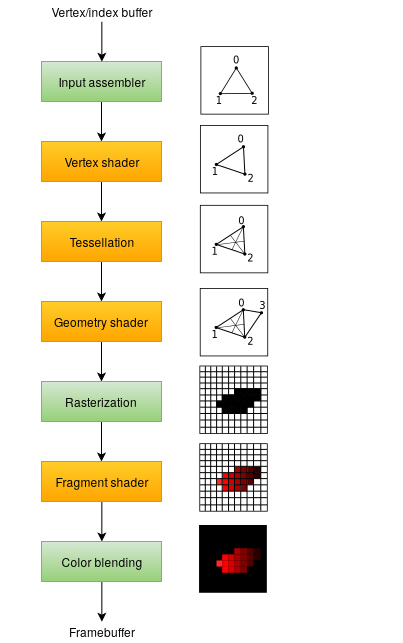
\includegraphics[scale=0.5, keepaspectratio]{img/vulkan_simplified_pipeline.png}
    \caption{Diagrama del cauce gráfico en Vulkan con las etapas principales del cauce,
    las etapas amarillas son programables, las etapas verdes son únicamente configurables
    dentro del cauce de renderizado.}
    \label{figura:khronos}
\end{figure}

A continuación se explican las diferentes etapas mostradas en la imagen del cauce gráfico de Vulkan
y en la parte final de la definición del cauce gráfico se explicará el uso de las etapas programables
y las etapas de configuración.

\begin{itemize}
  \item El ensamblador de entrada recopila los datos de vértices sin procesar de los búferes que
  se especifiquen y también puede usar un búfer de índice para repetir ciertos elementos sin tener
  que duplicar los datos del vértices.
  
  \item El sombreador de vértices se ejecuta para cada vértice y generalmente aplica transformaciones
  para convertir las posiciones de vértice del espacio modelo al espacio de la pantalla. También pasa
  datos de vértices por el pipeline.

  \item Los sombreadores de teselación permiten subdividir la geometría según ciertas reglas para aumentar
  la calidad de la malla. Esto se usa a menudo para hacer que las superficies como las paredes de ladrillo
  y las escaleras se vean menos planas cuando están cerca.

  \item El sombreador de geometría se ejecuta en todas las primitivas (triángulo, línea, punto) y puede
  descartar o generar más primitivas que las que se ingresaron, mapa 1:n. Esto es similar al shader de teselación,
  pero mucho más flexible. Sin embargo, no se usa mucho en las aplicaciones actuales porque el rendimiento no es
  tan bueno en la mayoría de las tarjetas gráficas, excepto en las GPU integradas de Intel.

  \item La etapa de rasterización discretiza las primitivas en fragmentos. Estos son los elementos de píxel
  que rellenan en el framebuffer. Los fragmentos que quedan fuera de la pantalla se descartan y los atributos
  generados por el shader de vértices se interpolan a través de los fragmentos, como se muestra en la figura.
  Por lo general, los fragmentos que están detrás de otros fragmentos de otras primitivas también se descartan
  aquí debido a los tests de profundidad.

  \item El sombreador de fragmentos se invoca para cada fragmento que sobrevive y determina en qué framebuffer (s)
  se escriben los fragmentos y con qué valores de color y profundidad. Puede hacerse utilizando los datos interpolados 
  del shader de vértices, que pueden incluir elementos como coordenadas de textura y normales para la iluminación.

  \item La etapa de mezcla de colores aplica operaciones para mezclar diferentes fragmentos que se asignan al mismo píxel
  en el framebuffer. Los fragmentos pueden simplemente sobrescribirse entre sí, sumarse o mezclarse en función de la transparencia.

\end{itemize}

Las etapas de función fija permiten ajustar las operaciones utilizando parámetros, pero la forma en que funcionan está predefinida.
Las etapas programables pueden cargar código en la tarjeta gráfica para aplicar exactamente las operaciones que se deseen y
optimizar las operaciones en los recursos de la tarjeta.  La etapa de sombreadores de fragmentos, por ejemplo, utiliza esta
clase de programas para implementar desde texturizado e iluminación, para dar un valor final de color de los fragmentos.
Estos programas se ejecutan en muchos núcleos de GPU simultáneamente para procesar muchos objetos y su conjunto de vértices
y fragmentos en paralelo.
\bigbreak
El pipeline (procesamiento en serie) de gráficos en Vulkan es casi completamente inmutable, por lo que debe recrearse el
pipeline desde cero si se desea cambiar los sombreados o enlazar diferentes framebuffers. La desventaja es que se deben
crear varios pipelines que representen todas las diferentes combinaciones de estados que se desean usar en las operaciones
de renderizado, sin embargo, debido a que todas las operaciones que se realizan en el pipeline se conocen de antemano,
el driver puede optimizar el renderizado mucho mejor.
\bigbreak
Algunas de las etapas programables son opcionales en función de lo que pretende hacer. Por ejemplo, las etapas de
teselación y geometría se pueden deshabilitar si solo se está dibujando una geometría simple. Si solo interesan
los valores de profundidad se puede deshabilitar la etapa de sombreado de fragmentos, que es útil para la generación
de mapas de sombras.

\subsubsection{Operaciones con Vulkan} 
\label{subsubsec:OpVulkan}

La API facilita el trabajo del driver y pone el control del hardware en manos del desarrollador, por ejemplo,
en la sincronización y la gestión de la memoria. Una de las ventajas de Vulkan frente a otras librerías gráficas
es su capacidad para depuración de los programas que se ejecutan en la tarjeta gráfica facilitando y agilizando
el desarrollo de las aplicaciones y la abstracción al desarrollador del hardware y los drivers con los que esté
trabajando. La arquitectura de Vulkan está desarrollada por capas y las herramientas de desarrollo son concebidas
como capas de la API. Grandes compañías de videojuegos como Valve o ID Software están utilizando esta librería
para el desarrollo de sus videojuegos. Es apreciable el aumento del rendimiento para un mismo hardware y una misma
aplicación haciendo uso de esta librería gráfica en lugar de otras especificaciones. 
\bigbreak
En la versión de Vulkan 1.1 se han añadido funcionalidades para protección de memoria restricciones de copia de
recursos en el renderizado y protección de contenido multimedia o procesamiento de imagen, además de ofrecer
un conjunto de operaciones paralelas de forma nativa en las etapas de shaders del cauce gráfico. Con estas nuevas
operaciones paralelas se consiguen nuevas formas de comunicación y compartición de memoria al realizar las operaciones
en la GPU de forma paralela.

\begin{figure}[hbt!]
    \centering
    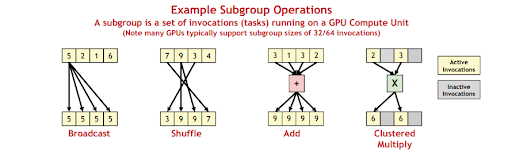
\includegraphics[scale=0.75, keepaspectratio]{img/vulkan_op.png}
    \caption{Imagen de grupo khronos de las operaciones paralelas soportadas de forma nativa en el lenguaje de shaders de Vulkan.}
    \label{figura:khronos}
\end{figure}

En la especificación de Vulkan se pueden encontrar el uso de vistas múltiples y realizar una única renderización
para el uso de múltiples pantallas.


\begin{itemize}
  \item Se puede hacer uso de grupos de dispositivos hardware heterogéneos de fabricantes diferentes que
  funcionan con un driver con Vulkan y mantienen de forma transparente los dispositivos al usuario de las tarjetas.
  
  \item Vulkan cuenta con funcionalidades de computación avanzada, fragmentos de memoria en 2 bytes, restricciones en
  los punteros a estructura de datos en memoria de la GPU y soporte para el desarrollo de núcleos aislados de
  procesamiento dentro del propio hardware.

  \item La especificación de Vulkan también es compatible con el programa de shaders de la librería gráfica de Microsoft
  HLSL, facilitando la portabilidad de un desarrollo hecho en Vulkan a DirectX 12.

  \item El lenguaje de shaders utilizado en Vulkan es SPIR-V y ofrece facilidades para la portabilidad de código escrito
  en SPIR-V a GLSL o HLSL para ser compatible tanto con OpenGL como con DirectX 12 facilitando la portabilidad de las
  aplicaciones y obtener shaders utilizando las mismas funcionalidades gráficas a un lengauje de programación de
  shaders HLSL o GLSL a SPIR-V.  Este trabajo de portabilidad de los lenguajes de shaders se hace a través del
  compilador de SPIR-V que es capaz de traducir de un lenguaje de shaders a otro HLSL, GLSL o SPIR-V. 
  
\end{itemize}

La especificación como todas la especificaciones de librerías gráficas del grupo Khronos está definida en la documentación
del estándar definiendo de forma explícita las funcionalidades obligatorias que deben de tener los fabricantes de las tarjetas
para poder cumplir con el estándar.


\subsection{Sistema de coordenadas en Vulkan} 
\label{subsec:SysVulkan}

Vulkan introduce una serie de cambios interesantes sobre OpenGL con algunos de los cambios clave de rendimiento y flexibilidad
que se mencionan. Un cambio más sutil pero igualmente importante para ser entendido es el del sistema de coordenadas.

\begin{figure}[hbt!]
    \centering
    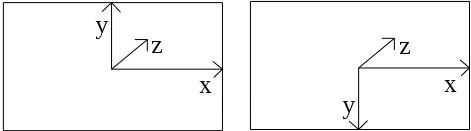
\includegraphics[scale=0.75, keepaspectratio]{img/coordinateDiagram.png}
    \caption{Cambio del sistema de coordenadas de OpenGL a la derecha al de Vulkan en la parte izquierda.}
    \label{figura:khronos}
\end{figure}

El primer cambio importante es que el eje y ahora apunta hacia abajo en la pantalla. Los ejes xz apuntan en la misma
dirección que antes. Esto significa que si no se corrige esto en los shaders portados de GLSL a SPIR-V sucederán dos
cosas importantes. En primer lugar, las imágenes se voltearán, hay múltiples formas de resolver esto. El método
utilizado en las muestras es simplemente agregar la siguiente línea a todos los programas de shaders vértices.

\begin{equation}
gl_Position.y = -gl_Position.y
\end{equation}

En OpenGL teníamos un espacio NDC a la izquierda, en Vulkan tenemos un espacio NDC a la derecha (suponiendo que el valor
de profundidad libre es 1, la función de profundidad es). \begin{equation} GL_LEQUAL / VK_COMPARE_OP_LESS_OR_EQUAL \end{equation}


El otro cambio en el sistema de coordenadas es el eje z, es decir, el rango de profundidad. En OpenGL el valor de profundidad
es un valor absoluto en un rango de [0, 1]. En Vulkan cambia a un valor relativo al vértice más lejano dentro de la ventana.
Para solucionar este problema y obtener los valores absolutos para etapas de face culling se utiliza la siguiente de línea
en la etapa de vértices de SPIR-V en Vulkan. 

\begin{equation}
gl_Position.z = (gl_Position.z + gl_Position.w) / 2.0
\end{equation}

Los trabajos futuros de esta especificación es seguir realizando herramientas de pruebas de calidad de la especificación
y priorizar las necesidades de los desarrolladores gráficos y conducir las nuevas tecnologías de futuras
generaciones de GPUs.

\section{DirectX} 
\label{sec:DirectX}

DirectX es la especificación de la librería gráfica de Microsoft de gráficos 2D y 3D. Esta especificación trata de realizar
una interfaz común para el trabajo en un sistema operativo de Microsoft, teniendo en cuenta la heterogeneidad del hardware de GPUs.

\subsection{Introducción a DirectX} 
\label{subsec:IntroDirectX}

Microsoft lanza su propia especificación para que los fabricantes puedan vender sus tarjetas gráficas en sistemas operativos Windows
implementando la especificación de DirectX en el driver de sus tarjetas gráficas. Microsoft realiza la especificación teniendo en
cuenta las tecnologías de las nuevas generaciones de GPUs que aparecen en el mercado, añadiendo nuevas funcionalidades en la
especificación de la librería, actualmente la versión más reciente de la especificación es la DirectX 12 compatible con la
especificación Vulkan del grupo Khronos.
\bigbreak
La tecnología de DirectX está pensada como un conjunto de API’s y cada una de ellas se encarga de realizar un trabajo
independiente de computación gráfica. La librería DirectX Math se encarga de realizar las operaciones matemáticas
sobre vectores o matrices de coma flotante. Las librerías Direct2D y Direct3D se encargan de realizar las renderizaciones
de modelos de gráficos en 2D y 3D respectivamente. También existen librerías para realizar programas compatibles con
versiones antiguas de Windows o hardware que no soporta la nueva especificación de la librería gráfica Classic DirectX
Graphics. Por otro lado Microsoft ha desarrollado una API específica para la entrada de dispositivos en este caso para su
mando de la XBox, XInput y una librería para procesamiento de señales de audio XAudio2. Además cuenta con una librería
de herramientas para depuración diagnóstico y compilación de su lenguaje de shaders HLSL.

\subsection{Sistema de coordenadas en Direct3D} 
\label{subsec:SysDirectX}

Direct3D utiliza un sistema de coordenadas levógiro. Si se están realizando acciones de transformación de una aplicación 
basada en un sistema de coordenadas dextrógiro, se debe realizar dos cambios en los datos  pasados ​a Direct3D de las
geometrías y operaciones de rotación o traslación.

\begin{figure}[hbt!]
    \centering
    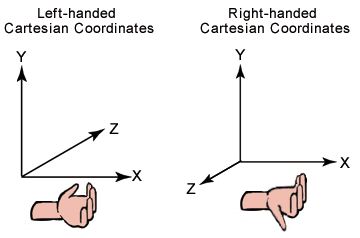
\includegraphics[scale=0.95, keepaspectratio]{img/leftrght.png}
    \caption{Uso de sistema de coordenadas levógiro y dextrógiro. Direct3D hace uso del primero como sistema de coordenadas.}
    \label{figura:khronos}
\end{figure}

Direct3D utiliza tres transformaciones para cambiar las coordenadas de un modelo 3D en coordenadas de píxeles (espacio de pantalla).
Estas transformaciones son transformaciones del mundo, transformaciones de vista y transformaciones de proyección.

\begin{itemize}
  \item La etapa de world transformation controla cómo las coordenadas del modelo se transforman en coordenadas absolutas.
  La etapa transformation world puede incluir traslaciones, rotaciones y escalas, pero no se aplica a las luces.
  
  \item La etapa de view transformation controla la transición de las coordenadas absolutas al "espacio de la cámara",
  determinando la posición de la cámara en el mundo.

  \item La etapa projection transform cambia la geometría del espacio de la cámara al "espacio de clip" y aplica
  distorsión de perspectiva. El término "espacio de clip" se refiere a cómo se recorta la geometría al volumen
  de la vista durante esta transformación descartando las primitivas de la geometría que no son visibles.
  
\end{itemize}

Finalmente, la geometría en el espacio del clip se transforma en coordenadas de píxeles (espacio de pantalla).
Esta transformación está controlada por la configuración de la ventana gráfica.

\begin{figure}[hbt!]
    \centering
    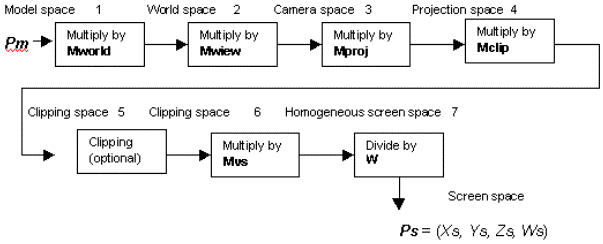
\includegraphics[scale=0.40, keepaspectratio]{img/d3dxfrm61.png}
    \caption{Etapas de transformación de los vértices en el cauce gráfico de OpenGL hasta la coordenada final
    del pixel de renderizado de la geometría por pantalla}
    \label{figura:khronos}
\end{figure}

La etapa de recorte de vértices y las etapas de transformación deben tener lugar en un espacio homogéneo (simplemente,
espacio en el que el sistema de coordenadas incluye un cuarto elemento), pero el resultado final para la mayoría de
las aplicaciones debe ser coordenadas tridimensionales (3D) no homogéneas definidas en el espacio de "pantalla".
Esto significa que tanto los vértices de entrada como la geometría de recorte deben traducirse en un espacio homogéneo
para realizar el recorte o clipping y luego volver a traducirse en un espacio no homogéneo para su visualización.

\subsection{Cauce gráfico en Direct3D 12} 
\label{subsec:CauceDX12}

El cauce gráfico programable Direct3D 12 aumenta significativamente el rendimiento de renderizado en comparación
con las interfaces de programación gráfica de la generación anterior.

\begin{figure}[hbt!]
    \centering
    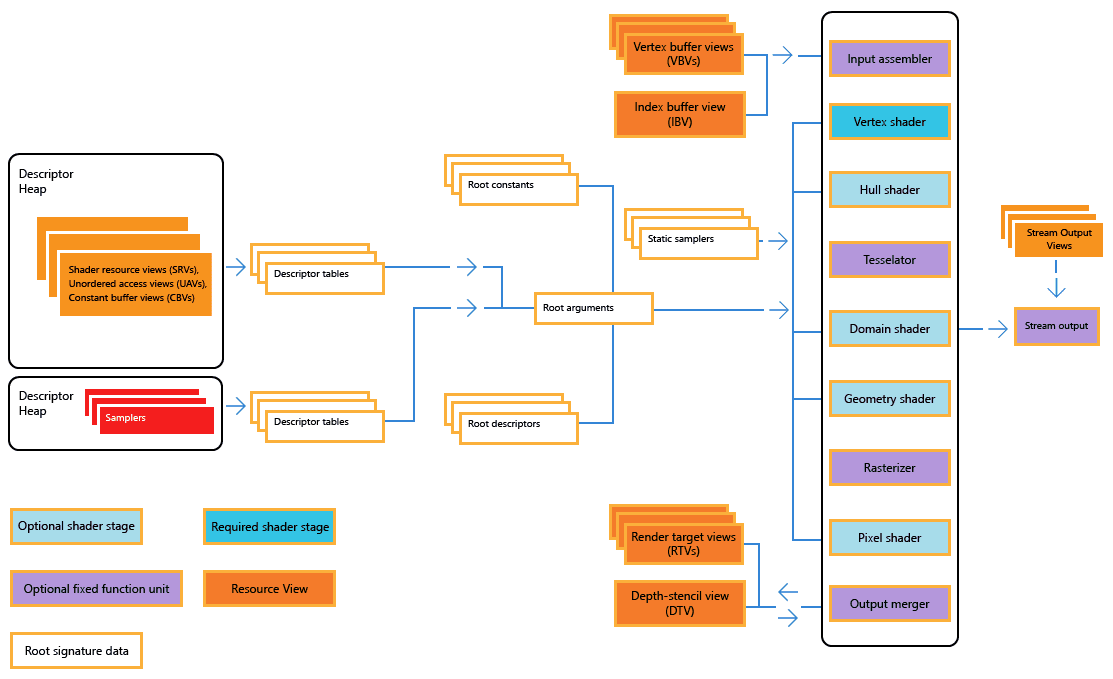
\includegraphics[scale=0.40, keepaspectratio]{img/pipelined123d.png}
    \caption{Diagrama de ilustración del cauce gráfico y estado de los gráficos en Direct3D 12.}
    \label{figura:khronos}
\end{figure}

Un cauce gráfico es un flujo secuencial de entradas y salidas de datos a medida que la GPU procesa los datos.
Dado el estado de la tubería y las entradas, la GPU realiza una serie de operaciones para crear las imágenes resultantes.
Una canalización de gráficos contiene shaders, que realizan cálculos y efectos de representación programables, y operaciones
de funciones fijas. Algunas operaciones del cauce son configurables. 

Una de las diferencias de DirectX 12 respecto a versiones anteriores es el uso de PSO objetos de estado en lugar de la
máquina de estados global del cauce gráfico para guardar el contexto.

\subsubsection{Cauce gráfico con objetos con estado PSO} 
\label{subsubsec:PSO}

Direct3D 12 presenta el objeto de estado de canalización (PSO). En lugar de almacenar y representar el estado del pipeline
en una gran cantidad de objetos de alto nivel, los estados de los componentes de la tubería como el ensamblador de entrada,
el rasterizador, el sombreador de píxeles y la fusión de salida se almacenan en un PSO. Un PSO es un objeto de estado de
canalización unificado que es inmutable después de la creación. 

El PSO seleccionado actualmente se puede cambiar de forma rápida y dinámica, y el hardware y los controladores pueden
convertir directamente un PSO en instrucciones de hardware y estado nativo, preparando la GPU para el procesamiento
de gráficos. Para aplicar un PSO, el hardware copia una cantidad mínima de estado precalculado directamente en los
registros del hardware. Esto elimina la sobrecarga causada por el controlador de gráficos que vuelve a calcular
continuamente el estado del hardware en función de todas las configuraciones de canalización y representación actualmente
aplicables. El resultado es una reducción significativa de la sobrecarga de llamadas de extracción, un mayor rendimiento
y más llamadas de extracción por trama.

El PSO aplicado actualmente define y conecta todos los sombreadores que se utilizan en la canalización de renderizado.
El lenguaje de sombreado de alto nivel de Microsoft (HLSL) está precompilado en objetos de sombreado, que luego se utilizan
en tiempo de ejecución como entrada para objetos de estado de canalización.

\begin{figure}[hbt!]
    \centering
    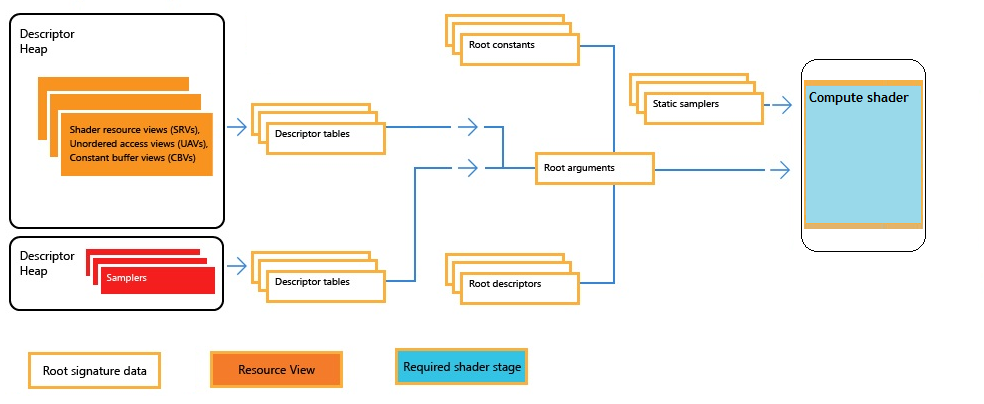
\includegraphics[scale=0.40, keepaspectratio]{img/compute-pipeline.png}
    \caption{El siguiente diagrama ilustra el cauce gráfico Direct3D 12 y su estado.}
    \label{figura:khronos}
\end{figure}

No hay unidades de funciones fijas en esta tubería, sin embargo, la memoria del heap de descriptores muestreos y muestreadores
estáticos todavía están disponibles en el cómputo.

\section{OpenGL} 
\label{sec:OpenGL}

OpenGL es una interfaz de programación que abstrae al desarrollador del hardware o GPU utilizada en su desarrollo.
OpenGL está pensado como una librería de gráficos para desarrolladores de videojuegos o simuladores de entornos virtuales. 

La librería viene con una serie de funciones que aprovechan las características de las especificaciones del estándar.
El hardware debe proveer al usuario de un driver que cumpla con las especificaciones de OpenGL para poder aprovechar
sus características de cómputo gráfico. 

OpenGL funciona en sistemas operativos Linux y MacOS y también funciona en sistemas operativos Windows al ser una
especificación que debe seguir el fabricante del driver de la tarjeta gráfica y no depender del sistema operativo.

La API OpenGL facilita el desarrollo de aplicaciones multiplataformas pudiendo desplegar el proyecto realizado en
diferentes entornos hardware que cumplan con la especificación del estándar en algunas o en la totalidad de sus
versiones de OpenGL.

\subsection{Introducción a OpenGL} 
\label{subsec:IntroOpenGL}

En las versiones anteriores de OpenGL 3.3, la especificación no daba una flexibilidad a los desarrolladores, era una
especificación más simple donde el driver era el encargado de realizar la mayoría de las tareas de computación
gráfica pero de manera poco eficiente, en las nuevas especificaciones de OpenGL se deja más libertad al desarrollador
pudiendo interferir en el núcleo del cauce de procesamiento gráfico, dando más flexibilidad y aumentando la eficiencia
de las aplicaciones gráficas. Estos dos modelos de programación son lo que se denominan modo inmediato y modo perfilado
del núcleo siendo el segundo el usado en las nuevas especificaciones de la API. En el uso del modo perfilado del núcleo
a partir de OpenGL 3.3, las versiones posteriores únicamente añaden nueva funcionalidad y eficiencia sin cambiar el
modelo de programación por este motivo se ha decidido realizar el proyecto utilizando la versión de OpenGL 3.3.

Es posible utilizar funcionalidades que soporte el fabricante de la tarjeta gráfica fuera de la especificación de OpenGL
como extensiones. Cuando una extensión se hace popular o es realmente útil a la hora de realizar un procesamiento o
técnica gráfica es añadida a la especificación de OpenGL, sin embargo a la hora de la implementación podemos añadir
extensiones y comprobar que en la plataforma donde se va a utilizar la extensión el driver la soporta y en tal caso
utilizarla o si no realizar el algoritmo gráfico a la manera antigua o legacy.

OpenGL está pensada como una máquina de estados, esta máquina de estados es lo que se denomina el contexto de OpenGL.
La máquina de estados está definida como un conjunto de variables que determinan cuál va a ser el comportamiento de OpenGL.
La idea del uso del contexto es cambiar la máquina de estados a través de variables añadiendo opciones y renderizar usando
el contexto actual de la máquina de estados. Muchas de las funciones de OpenGL son utilizadas únicamente para realizar un
cambio en la máquina de estados de la que luego beneficiarse a la hora de realizar la renderización de los objetos.

La especificación de OpenGL debe estar escrita en C, los drivers de los fabricantes de tarjetas gráficas que han seguido
las especificaciones de OpenGL han desarrollado el driver en C y por tanto no cuentan con características de lenguajes
de alto nivel, para solucionar este problema OpenGL cuenta con abstracciones para el uso de objetos a través de estructuras de datos.

Para terminar comentar que un objeto de OpenGL que utilizaremos en el desarrollo del proyecto son un subconjunto de estados
de OpenGL y que representan una entidad como puede ser la ventana de OpenGL donde podemos modificar algunos atributos del
objeto como su tamaño, la cantidad de colores que soporta la ventana o si la ventana es panorámica o no, entre otras
propiedades de la entidad ventana.

Una vez explicado OpenGL en el siguiente apartado se define la estructura dinámica de ejecución de OpenGL dentro de la máquina
de estados y el paso de una estructura de datos de una geometría en 3D a valores entendibles por la pantalla en la fase final
de renderizado del objeto pixelado.

\subsection{El cáuce gráfico de OpenGL} 
\label{subsec:CauceOpenGL}

El cauce gráfico de OpenGL se inicia cuando se quiere renderizar algún objeto 3D por pantalla esta transformación de renderizado,
pasar de un objeto geométrico 3D a un conjunto de valores RGB como parte final del renderizado se realiza a través de un pipeline
definido por etapas.

El cauce gráfico está dividido en dos grandes etapas divididas en etapas más especializadas. La primera etapa se pasa de un objeto
o geometría en un espacio de coordenadas en 3D a un objeto plano 2D. En la segunda etapa del cauce se rellenan los píxeles de la
pantalla con los colores de la parte final de los objetos ya en 2D de la etapas previas del cauce.

Cada etapa del cauce cuenta con una entrada de datos y una salida procesada que será la entrada de la siguiente etapa del cauce
hasta obtener un valor final de renderizado y rellenar los píxeles de pantalla con un valor RGB.

\begin{figure}[hbt!]
    \centering
    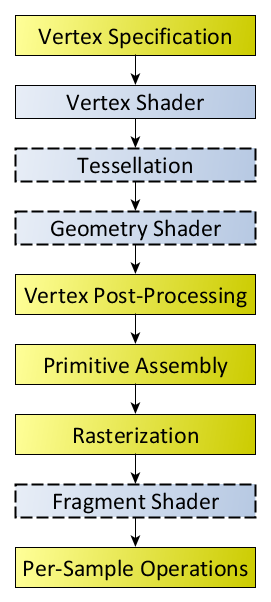
\includegraphics[scale=0.40, keepaspectratio]{img/RenderingPipeline.png}
    \caption{Imagen del cauce gráfico de OpenGL en sus diferentes etapas del cauce gráfico hasta la renderización.}
    \label{figura:khronos}
\end{figure}

Cada una de las etapas del cauce está especializada en una tarea (tienen una función específica), de esta manera es fácil
paralelizar la entrada de datos con operaciones SIMD (Single Instruction Multiple Data) y utilizar la arquitectura masivamente
paralela de una GPU. Cada etapa del cauce realizará el procesamiento paralelo con los datos de entrada, dependiendo de la
flexibilidad de la etapa se podrán realizar programas implementando algoritmos gráficos definidos por el desarrollador,
estas etapas más flexibles del cauce son las etapas programables mientras que otras etapas son únicamente etapas configurables.


\begin{itemize}
  \item Los programas que se desarrollan y ejecutarán en la GPU con los datos de entrada del cauce anterior se denominan programas
  de shaders y existen en todas las librerías de gráficos.
  
  \item Las etapas del cauce de la especificación de OpenGL están definidas como etapas que se denominan primitivas hasta las etapas
  finales de renderizado igual que ocurre en otras librerías gráficas.
\end{itemize}

En la primera etapa la etapa de especificación de vértices, se define una lista ordenada de límites o primitivas que serán el conjunto
total de los datos. Estos datos son representados en forma de atributos, como subconjunto de datos, cada subconjunto de datos
representa un vértice de la primitiva.

El conjunto total de atributos o vértices se denomina VAO (Vertex Array Object). Un ejemplo de definición de primitivas o array de
vértices puede tener un total de dieciocho valores, si definimos el valor de medida de un atributo en tres unidades, OpenGL
interpretará que tiene seis vértices dentro buffer de vértices representado por tres datos que en las siguientes etapas del
cauce se definirá como un vector de tres dimensiones. El valor del conjunto de atributos es arbitrario en esta etapa, es en las
siguientes etapas de vértices donde esta definición de atributo tiene un sentido espacial.

Una vez terminada la especificación del buffer de vértices en la CPU se realiza el renderizado de vértices con la llamada de
función de pintar primitivas de OpenGL glDrawArrays y comienzan a procesarse las diferentes etapas del cauce dentro de la GPU.

La siguiente etapa importante del cauce ya dentro del procesamiento de la GPU es la etapa de shaders de vértices, una etapa
programable del cauce. 

\begin{itemize}
  \item La etapa realiza un procesamiento básico sobre cada vértice de forma individual y define un valor de salida de vértice
  definido por el procesamiento del programa de shaders realizado por el desarrollador. 
  
  \item Las salidas están definidas por el desarrollador pero siempre espera una salida para cada atributo de entrada, mapeado 1:1
  la entrada y salida de vértices, esto se debe a que no pueden compartirse estados entre vértices por propósitos de rendimiento
  en el paralelismo del procesamiento de los mismos.
\end{itemize}

La etapa de shader de geometrías sigue trabajando a nivel de primitivas, devolviendo a su salida un valor nulo o un mayor número de
salidas de primitivas, 0:N, esta etapa también es una etapa programable del cauce.

\begin{itemize}
  \item Permite al desarrollador generar un mayor número de primitivas o eliminar algunas de ellas, de esta manera se puede conseguir
  una mejor definición de las primitivas homogéneas o similares en el procesamiento de la GPU y conseguir un mejor rendimiento en la
  definición de la geometría.
  
  \item Puede cambiar la definición de la primitiva inicial de un punto una línea o triángulo a cada una de ellas, respectivamente.
\end{itemize}

Una vez finalizada la etapa de geometrías empiezan las siguientes etapas del cauce gráfico relacionadas con el post procesamiento
de los vértices o primitivas.

\begin{itemize}
  \item La etapa de clipping o recorte, se encarga de separar las primitivas en un subconjunto de primitivas que están dentro de la
  ventana y de la perspectiva eliminando las primitivas interiores del volumen que no pueden ser vistas en el renderizado final,
  teniendo como referencia la matriz de vista del modelo proyectado generalmente por una cámara.
  
  \item En la etapa de ensamblado de las primitivas, dada una entrada de vértices se realiza la serialización de las primitivas
  definidas por el usuario en las etapas anteriores, si se definieron 12 vértices como un array de triángulos en esta etapa se
  generarán 10 triángulos en base a la definición previa de la primitiva básica y el orden de definición de los vértices de la
  primitiva, ya sea por orden de entrada o por el orden definido en un array de índices de la primitiva.

  \item Existe una última operación en el post procesamiento de vértices, etapa de culling, esta etapa se encarga de descartar las
  primitivas finales que no estén dentro de la ventana proyectada por la cámara, evitando el cómputo innecesario de primitivas en
  el renderizado final de los fragmentos.

  \item En la etapa de rasterización las primitivas son rasterizadas en el orden que entran por esta etapa dividiendo las primitivas
  en una estructura de datos denominados fragmentos.
\end{itemize}

Un fragmento es un conjunto de estados que se utiliza para calcular los datos finales de un pixel o de una muestra si se tiene
habilitado el MSAA (Multiple Sampling Anti Aliasing) en el framebuffer de salida. El estado del fragmento incluye su posición
en el espacio de la pantalla y una lista de datos arbitrarios que se obtuvieron del vértice o en la etapa de shaders de geometrías
después de pasar por la etapa de rasterización.


\begin{itemize}
  \item En la etapa de shaders de fragmentos se realiza un procesamiento sobre los fragmentos. La salida de la etapa de fragmentos es
  un valor de color dado a cada fragmento, incluyendo un valor de profundidad del fragmento previo.  En esta etapa tenemos control
  del valor de salida tanto de profundidad como de color final del fragmento. 
  
  \item La etapa de fragmentos es una etapa programable y es un etapa opcional, si no se define un programa de shaders para la etapa
  de fragmentos el valor de renderización final es el buffer de profundidad, calculado por el posicionamiento de las primitivas de
  las etapas anteriores.

  \item Las etapas de fragmentos realizan una serie de operaciones por pixel o muestra. Estas etapas están definidas por un conjunto
  de tests que son aplicados a los fragmentos, si el test falla el fragmento se descarta, no se renderiza en pantalla, algunos de
  estos tests más importantes son el test de profundidad para no pintar objetos superpuestos, haciendo uso del valor de profundidad
  de los fragmentos.
\end{itemize}

La última parte del cauce realiza una serie de test sobre los fragmentos decidiendo si el fragmento se renderiza o no por pantalla en
su posterior valor a pixel de pantalla.

\begin{itemize}
  \item  La etapa de transparencia de color realiza la operaciones de test para cada color de fragmento, se realizan una serie de
  operaciones lógicas entre el fragmento y el framebuffer de colores permitiendo el paso de color entre objetos y poder renderizar
  materiales que puedan ser transparentes.
\end{itemize}

Por último el fragmento es escrito en el framebuffer de salida que está estructurado por los canales de color y profundidad y mostrando
finalmente la renderización final al usuario por pantalla.

\subsection{Sistema de coordenadas en OpenGL} 
\label{subsec:SysOpenGL}

Por convención, OpenGL es un sistema dextrógiro. Lo que esto básicamente dice es que el eje x positivo está a su derecha, el eje y
positivo está hacia arriba y el eje z positivo está hacia atrás. Pensando en la pantalla como el centro de los 3 ejes y el eje z positivo
que atraviesa la pantalla hacia el usuario del ordenador. Los ejes se dibujan de la siguiente manera:

\begin{figure}[hbt!]
    \centering
    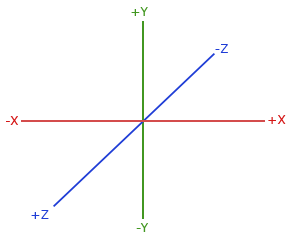
\includegraphics[scale=0.40, keepaspectratio]{img/coordinate_systems_right_handed.png}
    \caption{Sistema de coordenadas en OpenGL}
    \label{figura:khronos}
\end{figure}

Para entender por qué se llama dextrógiro, se debe hacer lo siguiente:

\begin{itemize}
  \item Estirar el brazo derecho a lo largo del eje y positivo con la mano hacia arriba.
  \item Dejar el pulgar apuntando a la derecha.
  \item Dejar que el dedo índice señalar hacia arriba.
  \item Doblar el dedo medio hacia abajo 90 grados.
\end{itemize}

Si se sigue ese procedimiento, el pulgar debe apuntar hacia el eje x positivo, el dedo índice hacia 
el eje y positivo y el dedo medio hacia el eje z positivo. Si se hace esto con el brazo izquierdo,
el eje z está invertido. Esto se conoce como un sistema levógiro y es utilizado comúnmente por DirectX.
Hay que tener en cuenta que en las coordenadas de dispositivo normalizadas, OpenGL en realidad usa un
sistema zurdo, la matriz de proyección cambia la mano al modo dextrógiro.

\section{Entorno y herramientas} 
\label{sec:Entorno}

A continuación se nombran las implementaciones abiertas de la librería de OpenGL, entorno y herramientas 
utilizadas para el proyecto, en este caso el uso de glfw3 con glad y la ayuda de la librería de matemática
para gráficos compatible con la especificación OpenGL, GLM (OpenGL Mathematics Library).

\subsection{Glad} 
\label{subsec:Glad}

Esta es una herramienta para generar cargadores de funciones OpenGL. Selecciona el lenguaje, las versiones
de OpenGL / OpenGL ES, los perfiles principales o compatibles, y los genera en un fichero de cabecera.

La herramienta genera el fichero de cabecera con las declaraciones de la interfaz de las funciones GL y
las estructuras de datos para la versión de GL que se elija, y genera un pequeño archivo fuente C que
resuelve todas las funciones en tiempo de ejecución para ayudar al compilador en la definición de
símbolos y tipos de datos de las funciones de la librería de OpenGL antes de enlazar con la librería
gráfica binaria instalada en el sistema operativo y generar el fichero binario de la aplicación gráfica
definida por el desarrollador.

A la hora de definir los includes en el programa con la definición de las funciones de la librería de
OpenGL se debe cargar primero el fichero de cabecera generado por la herramienta GLAD para resolver de
manera correcta las estructuras de datos y las definiciones de funciones de OpenGL en el entorno de
desarrollo.

\subsection{GLFW} 
\label{subsec:GLFW}

GLFW es una biblioteca multiplataforma de código abierto para el desarrollo de OpenGL, OpenGL ES y Vulkan,
en plataformas de escritorio. Proporciona una API simple para crear ventanas, contextos y superficies
gráficas y recibir entradas o eventos de los periféricos, está escrito en C y es compatible con los sistemas
operativos Windows, macOS y Linux.

Las ventajas de usar la librería GLFW con la implementación de algunos de los estándares gráficos son
las siguientes:

\begin{itemize}
  \item Se puede obtener una ventana y un contexto de OpenGL utilizando dos llamadas a la
  función de la API.

  \item Soporta OpenGL OpenGL ES, Vulkan y algunas de las opciones extendidas de las
  especificaciones.

  \item Soporta el uso de múltiples ventanas y múltiples monitores con alta densidad de
  píxeles o alta resolución (high-DPI).

  \item Tiene soporte para entradas de teclado ratón eventos de ventana y gamepad haciendo
  uso de polling sobre los dispositivos o utilizando manejadores de eventos, haciendo fácil
  el uso de periféricos dentro de las aplicaciones.

  \item La librería viene con tutoriales con código de ejemplo y documentación de las
  funciones de la API.

  \item Tiene acceso a objetos nativos en tiempo de compilación para características específicas
  de ciertas plataformas.

  \item Existe una comunidad que da soporte y mantiene la librería actualizada en diferentes
  lenguajes de programación.

\end{itemize}

La herramienta GLFW es la encargada de generar la entidad o ventana del contexto de OpenGL.

\subsection{OpenGL Mathematics Library GLM} 
\label{subsec:GLM}

OpenGL Mathematics (GLM) es una biblioteca matemática desarrollada en C++ solo para software
de gráficos basada en las especificaciones de OpenGL de su lenguaje de shaders Shading Language (GLSL).
GLM proporciona clases y funciones diseñadas e implementadas con las mismas convenciones de nombres
y funcionalidades que GLSL para que cualquiera que conozca GLSL, pueda usar la librería GLM también
en la CPU a través de lenguajes de programación cómo C++.

Este proyecto no se limita a las funciones GLSL. Un sistema de extensión, basado en las convenciones
de extensión GLSL, proporciona capacidades extendidas: transformaciones matriciales, cuaterniones,
empaquetamiento de datos, números aleatorios, ruido, etc. Por lo que muchas operaciones de lenguaje
de shaders que se ejecutan dentro de la GPU pueden ser portadas también a la CPU, utilizando esta librería.

Esta biblioteca funciona perfectamente con OpenGL pero también garantiza la interoperabilidad con otras
bibliotecas de terceros y SDK o librerías externas que no tengan que ver con OpenGL. Es un buen candidato
para la representación de software (trazado de rayos / rasterización), procesamiento de imágenes,
simulaciones físicas y cualquier contexto de desarrollo que requiera una biblioteca matemática gráfica.

GLM está escrito en C++ 98 pero puede aprovechar C++ 11 cuando es compatible con el compilador. Es una
biblioteca independiente de la plataforma y oficialmente admite la mayoría de los compiladores de C++
más utilizados en la industria.

\begin{figure}[hbt!]
    \centering
    
\includegraphics[scale=0.80, keepaspectratio]{img/logo_glm.png}
    \caption{Logotipo de la librería matemática compatible con las especificaciones del lenguaje GLSL.}
    \label{figura:logo_glm}
\end{figure}

\subsection{OpenGL Utility Libraries GLUT} 
\label{subsec:GLUT}


La librería glut es un conjunto de herramientas externas que trabajan con el core de OpenGL,
su finalidad es servir de interfaz con diferentes dispositivos de entrada y salida heterogéneos,
utilizados en el campo de realidad virtual.

Ahora se hablará de algunos de los motores gráficos que utilizan todas o algunas de estas
tecnologías para que el usuario pueda realizar aplicaciones gráficas de forma sencilla evitando
el uso de las librerías gráficas y paradigmas de programación vistos de bajo nivel.

\section{Motores Gráficos} 
\label{sec:Motores}

En este apartado realizaremos una introducción de tres de los motores gráficos más utilizados
en la actualidad; Unreal, Unity y Blender. Para realizar la simulación utilizaremos blender y
realizaremos una mayor profundidad en el uso de este motor gráfico en la fase final de resultados.

\subsection{Unreal} 
\label{subsec:Unreal}

Unreal es un motor gráfico desarrollado por la compañía Epic Games, sus primeras versiones fechan del año
1998, el desarrollo del motor está realizado en C++ y sus versiones son Open Source. Su página web cuenta
con una documentación de todas las funcionalidades del motor además de tutoriales. Unreal cuenta con una
comunidad activa que realizan aportaciones al desarrollo y diseño del motor además de preguntas a problemas
que puedan tener otros usuarios. El motor está pensado como un conjunto de módulos y herramientas para
facilitar la creación de contenido gráfico.

El desarrollo de las aplicaciones gráficas en Unreal puede desplegarse en multiplataforma, desde sistemas
operativos Windows hasta máquinas embebidas de realidad virtual de Valve o Samsung, teléfonos móviles o
consolas de manera gratuita. Unreal cobra por el uso de la plataforma el cinco por ciento de las aplicaciones que
superen una cuota de mercado mayor de 3000 dólares.

Entre las características principales del motor Unreal cuenta con un módulo de renderizado de gráficos, este
módulo se encarga de la simulación de luces, generación de sombras carga de materiales y texturas, efectos
de partículas o post procesado. Es decir la parte principal de renderización y visualización de las geometrías.

Cuenta con un módulo para el desarrollo de interfaces de usuario Unreal Motion Graphics User Interfaces UMG.
La interfaz de usuario hace uso de Widgets para la captura de eventos de usuario a través de botones barras
de progreso, menús etc. Esta interfaz interactiva ayuda al desarrollador a crear contenido de manera muy
sencilla y realizar cierta lógica de animación o jugabilidad sin tener conocimientos sobre programación.

Uno de los principales módulos de Unreal y más conocido con los Blueprint Visual Scripting. Este módulo
está diseñado como un diagrama de flujo o una máquina de estados presentado como un visualización en
bloques con un flujo de ejecución.

\begin{figure}[hbt!]
    \centering
    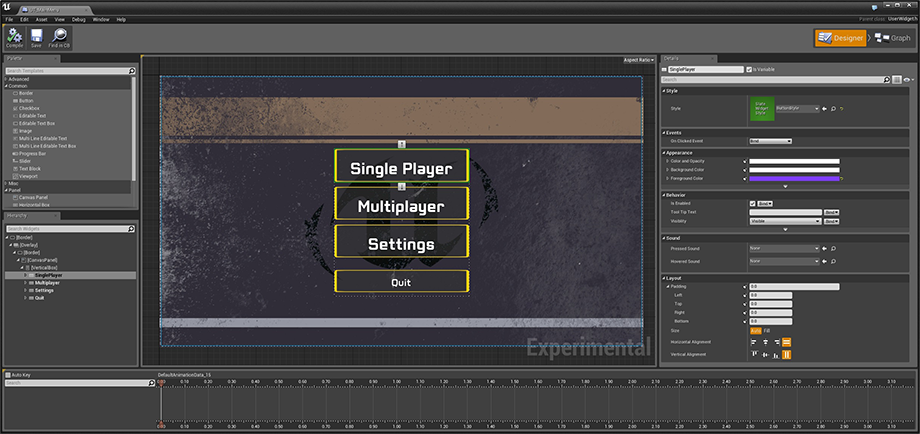
\includegraphics[scale=0.30, keepaspectratio]{img/menu_unreal.png}
    \caption{Uso de flujo de programa utilizando la interfaz blue visual scripting}
    \label{figura:menu_unreal}
\end{figure}

La idea es utilizar esta interfaz de visualización para usuarios con poca experiencia en programación
y poder generar comportamientos animaciones u objetos gráficos con materiales de manera rápida y
sencilla que solo podrían ser accesibles para desarrolladores o personas con conceptos de programación.

\begin{figure}[hbt!]
    \centering
    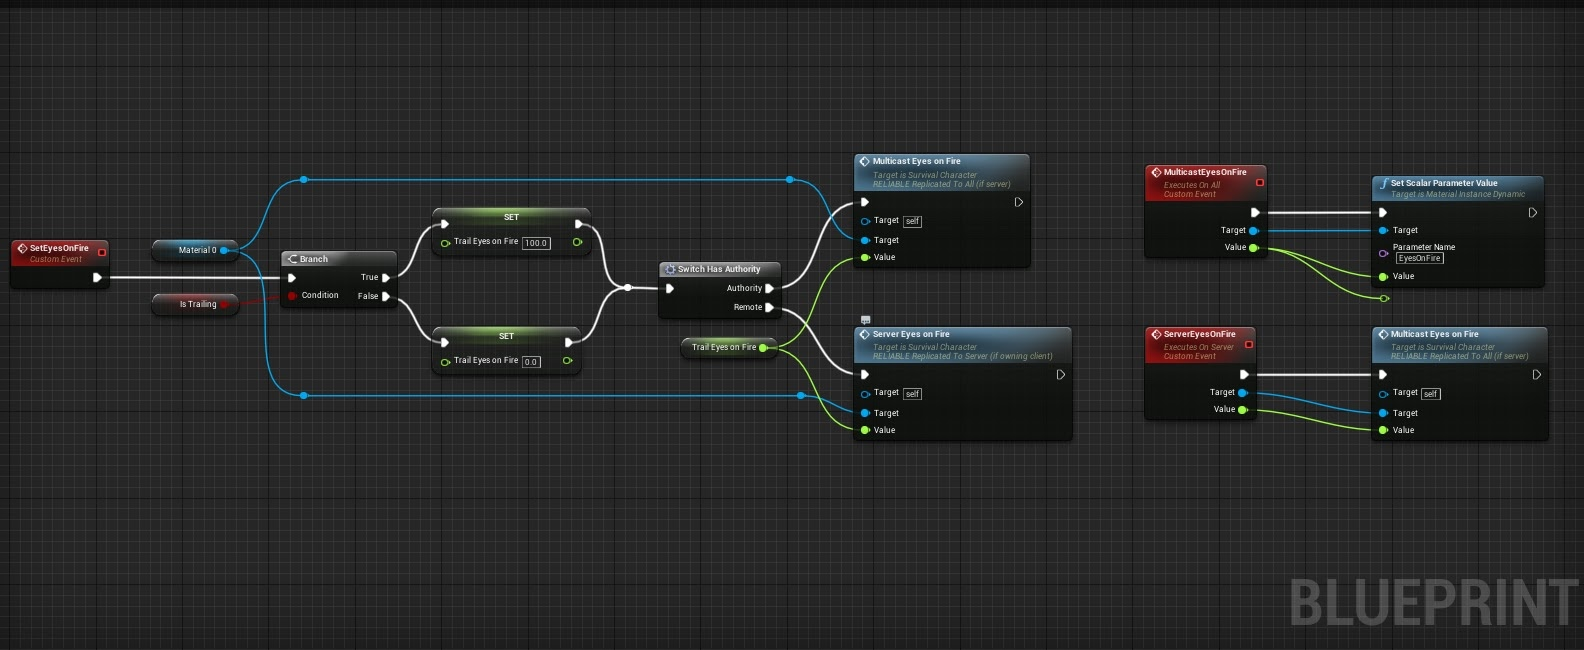
\includegraphics[scale=0.30, keepaspectratio]{img/option1_unreal.jpg}
    \caption{Uso de flujo de programa utilizando la interfaz blue visual scripting}
    \label{figura:option1_unreal}
\end{figure}

Hace uso de una API para realizar un flujo de ejecución y lógica de las aplicaciones, en lenguajes de
programación C++ y Luna. La API de C++ es clara y sencilla de utilizar aunque se deben tener conocimientos
previos de programación en este lenguaje para poder utilizar esta API. Esta dificultad puede ser resuelta
con el uso del módulo de  Blueprint Visual Scripting que utiliza por debajo la misma API del motor para
generar la lógica o flujo de ejecución de las animaciones.

Unreal trata de ser un motor gráfico genérico e innovador para la realización de contenido gráfico de
simulaciones virtuales o animación cinematográfica. El uso de lenguaje C++ como el uso del editor o
algunos módulos del motor requieren de un conocimiento previo del funcionamiento de físicas, geometrías
o materiales en entornos gráficos, esto dificulta la curva de aprendizaje de la plataforma.

Uno de los principales puntos fuertes de Unreal es su buen uso de los recursos, con una buena gestión
de la memoria y del cauce gráfico en el renderizado de los objetos o las físicas dentro de la plataforma
a pesar de su complejidad. 

El competidor directo de Unreal en el desarrollo de videojuegos multiplataforma en la actualidad es el
motor gráfico Unity 3D.

\subsection{Unity 3D} 
\label{subsec:Unity3D}

Unity es un motor gráfico pensado para el desarrollo de aplicaciones gráficas multiplataforma en tiempo
real. Sus principales usos son el desarrollo de videojuegos y la creación cinematográfica de animación.
La plataforma de Unity contiene partes gratuitas Open Source y otras privativas que pueden ser explotadas
con la adquisición de licencias con un coste adicional.

Unity cuenta con una interfaz potente para importar archivos externos heterogéneos y su uso dentro del
espacio de trabajo de un proyecto creado en Unity.  La importación de archivos cuenta con importación
de ficheros de audio y sonido, renderizados 3D realizados en otras plataformas de diseño gráfico como
autocad o malla o importación de fuentes de lenguaje e idiomas.

\begin{figure}[hbt!]
    \centering
    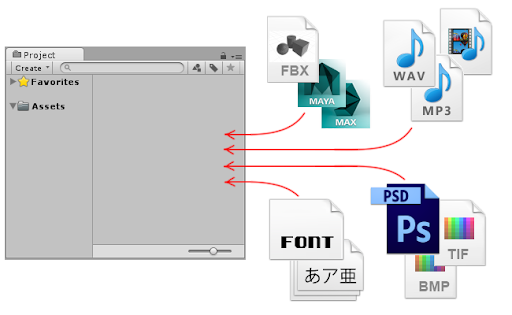
\includegraphics[scale=0.60, keepaspectratio]{img/unity_assets.png}
    \caption{Visualización del uso de la librería Assets para importación de archivos en Unity}
    \label{figura:unity_assets}
\end{figure}

Unity también cuenta con primitivas pre definidas para objetos geométricos básicos como esferas cubos
ellipses o planos, parecido al utilizado en el proyecto, haciendo uso de funciones matemáticas parametrizadas
para generar las primitivas, tamaños o formas de las superficies.

El foco de atención principal del usuario en Unity se hace a través de la ventana principal, dentro de
la ventana principal se pueden cargar en diferentes pasos el desarrollo de las aplicaciones gráficas,
es decir ventanas con funciones específicas del motor se cargan dentro de la ventana principal. 

En la ventana de proyecto se pueden manejar los materiales geometrías o archivos externos cargados con la
interfaz Assets. La ventana de proyecto se puede gestionar en un panel adicional donde está contenida la
estructura de directorios del proyecto y los ficheros importados. En la ventana de proyecto se puede cargar
una sub ventana en la que se pueden ver los tipos de archivos cargados en la estructura de directorios,
geometrías, texturas, programas de shaders de materiales, ficheros de audio etc.

La vista de escena en la ventana principal, muestra al usuario una visión interactiva del mundo creado con
Unity en la que se podrán editar las luces de la escena posición de los objetos y las cámaras. Esta vista
es fácil de manejar para los usuarios que utilizan por primera vez el motor de Unity y para hacerse una
idea del trabajo con el entorno de desarrollo.

En la vista de juego dentro de la ventana principal se podrá ver el resultado final de la aplicación gráfica
creada con Unity en la que deberemos ver la perspectiva desde cámaras de la escena y el renderizado en tiempo
real de la aplicación. 

En esta vista los cambios realizados de forma interactiva son temporales. Como la bajada de la resolución para
emular el uso de dispositivos antiguos o con menor poder computacional. La ventana además avisa al usuario si
no existen cámaras en la escena para advertir de que no hay ninguna vista que pueda ser utilizada por el módulo
de renderizado.

En la ventana de jerarquías podemos ver las dependencias que existen entre los objetos de la escena, algunos de
estos objetos pueden ser geometrías cargadas con la interfaz Asset o componentes del motor como luces o cámaras. 

La ventana de jerarquías nos da una visión del árbol de transformadas de Unity y de las dependencias de los
objetos dentro de la escena de manera global. En esta vista se pueden también crear las dependencias entre
los objetos creando nodos hijos de otro objetos y generar partes del árbol de jerarquía de la escena. Aunque
su uso principal es la visualización del árbol de jerarquía, en escenas de juego más complejas.

\begin{figure}[hbt!]
    \centering
    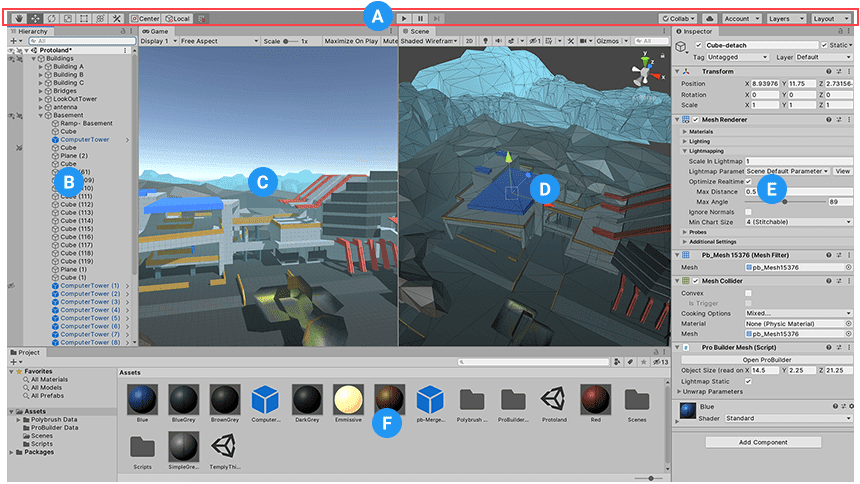
\includegraphics[scale=0.40, keepaspectratio]{img/editor_unity.png}
    \caption{Uso de ventanas en Unity}
    \label{figura:editor_unity}
\end{figure}

El uso de programación también es algo a tener en cuenta dentro de Unity. Muchas aplicaciones necesitan el uso
de de programas para responder a eventos de usuario en el momento que sea necesario, en los scripts es posible
realizar efectos gráficos control de físicas, comportamiento de los objetos o creación de un sistem de inteligencia
artificial personalizado para los objetos de juego. El uso de programación en Unity se realiza a través de la
API de Unity en C\#.

\begin{figure}[hbt!]
    \centering
    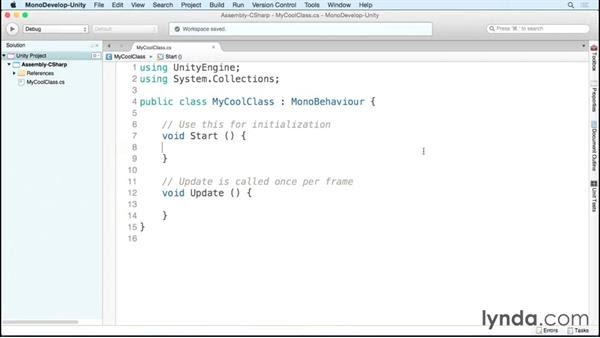
\includegraphics[scale=0.60, keepaspectratio]{img/APIUnity.jpg}
    \caption{Ejemplo de uso de lenguaje de scripting en Unity 3D de componentes}
    \label{figura:APIUnity}
\end{figure}

Unity es un motor con una curva de aprendizaje sencilla en el uso del editor, los conceptos del motor o uso de un
lenguaje de programación de componentes sencillo en C\#. El usuario puede ser capaz de realizar un prototipo de
juego o aplicación virtual de forma rápida. Con el uso del módulo Asset es fácil insertar contenidos de terceros
dentro del motor aunque puede que este contenido se quede corto cuando queremos realizar mundos algo más complejos. 

Los mayores problemas que podemos encontrar en Unity son la mala gestión de los recursos. Al estar implementados
algunos módulos en .Net es posible tener problemas de rendimiento en la gestión de la memoria con el recolector de basura. 

También se encuentran restricciones al no ser un motor completamente Open Source como Unreal, si se quiere realizar
alguna funcionalidad específica que no soporte el motor no se puede añadir.

La inestabilidad entre versiones intermedias también es un problema en Unity ya que en la realización de parches suelen
meterse regresiones y bugs nuevos dentro de la plataforma.

\subsection{Blender} 
\label{subsec:Blender}

Blender es un motor gráfico open source gratuito para la creación de mundos en 3D. El motor blender da soporte completo
para la creación en 3D desde el modelado, la animación, el renderizado, o el seguimiento de objetos. También es posible
realizar animaciones en 2D con blender. El motor blender soporta el cauce completo desde la creación de los objetos 3D
hasta la etapa final de renderizado. Blender se puede utilizar para crear visualizaciones en 3D, como imágenes fijas para
crear texturas, animaciones en 3D, tomas de efectos visuales y edición de video, se adapta bien a desarrollos individuales
y pequeños estudios que se benefician de su proceso unificado de desarrollo y respuesta.

El motor gráfico blender puede realizar desarrollos de aplicaciones gráficas multiplataforma que se ejecuta en sistemas Linux,
macOS y Windows. Blender también tiene requisitos de memoria y procesamiento relativamente pequeños en comparación con otras
plataformas de creación 3D. Su interfaz utiliza OpenGL para proporcionar una experiencia consistente en todo el hardware
y las plataformas compatibles con OpenGL. Tiene una amplia variedad de herramientas que lo hacen adecuado para casi cualquier
tipo de producción de medios, personas y estudios de todo el mundo que lo usan para proyectos de pasatiempos, comerciales y
largometrajes.


\begin{itemize}
  \item Blender es un conjunto de módulos para creación de contenido 3D totalmente integrado, que ofrece una amplia gama de
  herramientas esenciales, que incluyen modelado, renderizado, animación, edición de video, efectos visuales, composición,
  texturizado y muchos tipos de simulaciones.

  \item Es multiplataforma, con una interfaz gráfica de usuario OpenGL que es uniforme en todas las plataformas principales
  (y personalizable con scripts de Python).

  \item Tiene una arquitectura 3D de alta calidad, lo que permite un flujo de trabajo de creación rápido y eficiente.

  \item Cuenta con un apoyo activo de la comunidad, consulte blender.org/community para obtener una lista extensa de sitios.

  \item Tiene un pequeño ejecutable, que es opcionalmente portátil.
\end{itemize}


Blender hace posible realizar una amplia gama de tareas, y puede parecer desalentador cuando se trata de comprender los
conceptos básicos. Sin embargo, con un poco de motivación y el material de aprendizaje adecuado, es posible familiarizarse
con Blender después de algunas horas de práctica.

\begin{figure}[hbt!]
    \centering
    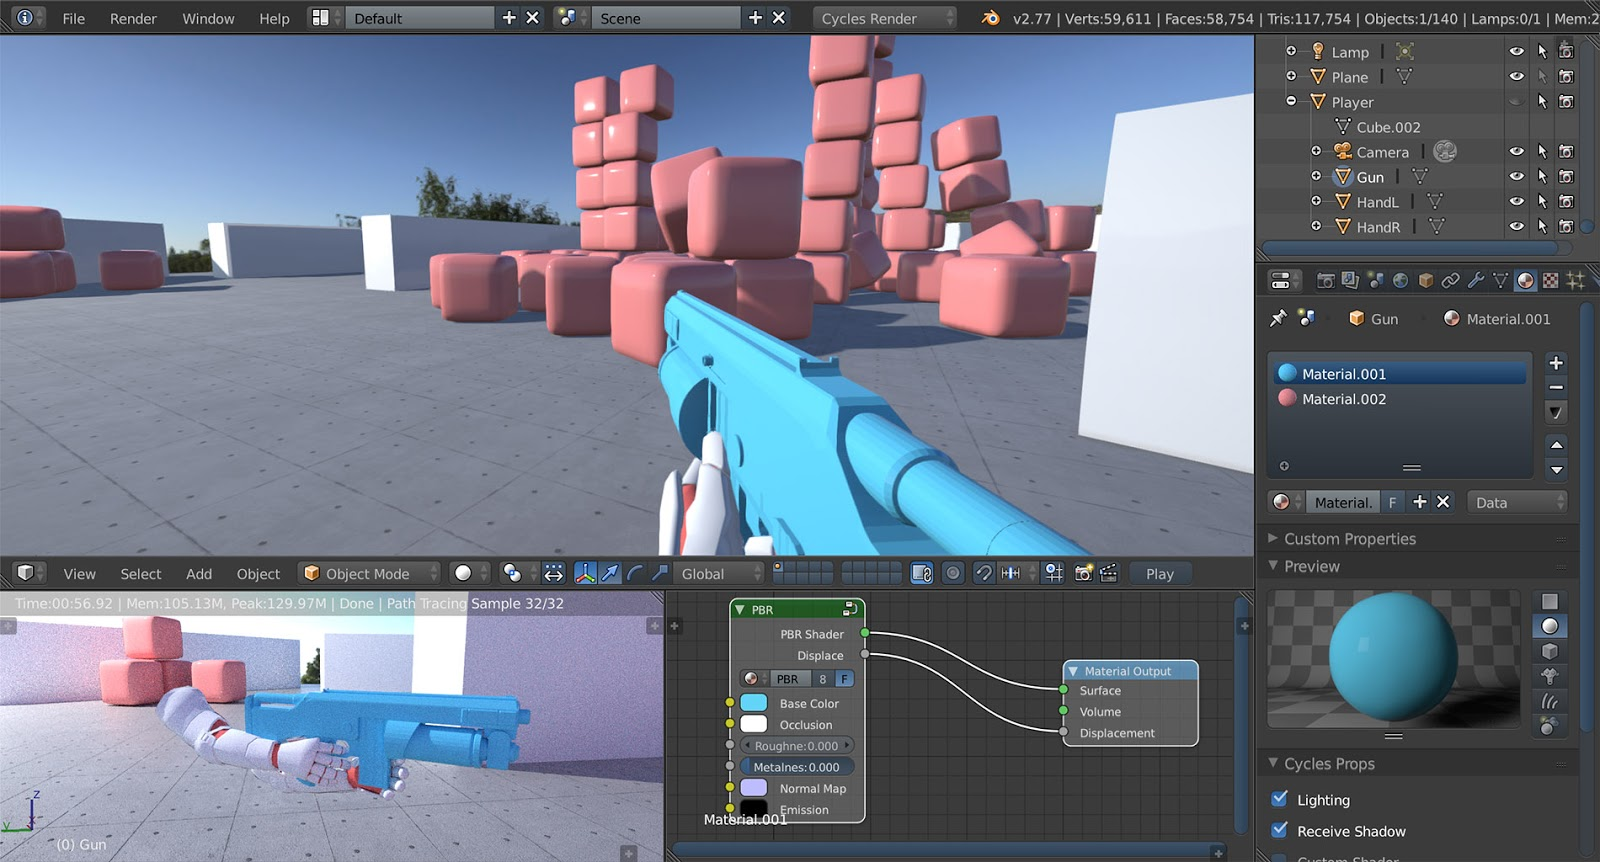
\includegraphics[scale=0.30, keepaspectratio]{img/Blender.jpg}
    \caption{Visualización general de ventanas en blender para la creación de una escena virtual.}
    \label{figura:Blender}
\end{figure}

En la imagen se puede observar: 

\begin{itemize}
  \item La ventana de renderización de la aplicación gráfica

  \item La definición de materiales a través de diagrama de bloques que termina
  convirtiendose en un programa de shader que ejecutará en la tarjeta gráfica.

  \item Ventana de aspecto final del efecto de material con iluminación

  \item El árbol de jerarquía de la escena con los diferentes objetos que la componen.

\end{itemize}

Una vez vistas las tecnologías y los diferentes motores gráficos que se encuentran actualmente en el mercado,
el uso de recursos o la realización de conceptos en los motores gráficos se pasará a ver su aplicación dentro
del desarrollo del motor gráfico del proyecto.


%%%%%%%%%%%%%%%%%%%%%%%%%%%%%%%%%%%%%%%%%%%%%%%%%%%%%%%%%%%%%%%%%%%%%%%%%%%%%%%%
%%%%%%%%%%%%%%%%%%%%%%%%%%%%%%%%%%%%%%%%%%%%%%%%%%%%%%%%%%%%%%%%%%%%%%%%%%%%%%%%
% DISEÑO E IMPLEMENTACIÓN %
%%%%%%%%%%%%%%%%%%%%%%%%%%%%%%%%%%%%%%%%%%%%%%%%%%%%%%%%%%%%%%%%%%%%%%%%%%%%%%%%

\cleardoublepage
\chapter{Arquitectura e implementación del motor gráfico}

El motor está diseñado como una API de alto nivel desarrollada en C++. La interfaz de la API cuenta con un conjunto
de clases públicas para definir abstracciones gráficas y métodos de estas clases para decidir el comportamiento del motor.

La arquitectura está formada por una estructura de datos principal en forma de árbol de nodos, los nodos del árbol
serán los objetos de juego, concepto obtenido del motor gráfico de Unity y Blender.

El diseño de la arquitectura está especificado en un patrón de diseño basado en componentes que formarán la estructura
principal del desarrollo del motor, siguiendo los principios de este diseño, utilizado en los motores Unity o Blender.
Para trabajar el cauce gráfico se utilizará una jerarquía de clases de dibujadores o Drawers que tendrán un comportamiento
de componente especial para saber que objetos de juego son renderizables y deben realizar las operaciones del cauce gráfico.

En la primera parte del desarrollo explicaremos la estructura estática de la arquitectura, la explicación de las clases que
definen las estructuras de datos del motor y las dependencias que existen entre ellas. 

En la segunda parte del desarrollo se explicará de forma detallada la estructura dinámica de la arquitectura explicando paso
a paso las fases de ejecución del motor.

La definición de la estructura estática y dinámica explicarán de forma detallada el funcionamiento del motor gráfico, las
abstracciones gráficas realizadas y la solución al cauce gráfico de OpenGL transparente para el usuario, utilizando técnicas
usadas en otros motores.

\section{Definición estática del motor} 
\label{sec:estatica}

Para definir las clases del motor se empezará por las clases de alto nivel que son utilizadas por el usuario para definir una
escena renderizable en una ventana de OpenGL, según vayan definiéndose las clases de alto nivel se entrará en detalle de las
clases que definen partes de las técnicas gráficas implementadas y su acceso a la interfaz de OpenGL.

La primera clase a explicar es la clase Engine, esta clase almacena la ventana de OpenGL, las instancias de teclado y reloj
para el manejador de eventos de entrada de polling de la interfaz de OpenGL y la escena renderizable dentro de la ventana.
En el constructor recibe como parámetro la escena creada por el usuario para su posterior renderizado en la ventana de OpenGL.
La clase motor cuenta con tres métodos públicos; inicialización actualizado y bucle principal.



\subsection{Arquitectura e implementación del motor gráfico} 
\label{sec:arquitectura}


figura~\ref{fig:arquitectura}.

\begin{figure}
  \centering
  \includegraphics[width=9cm, keepaspectratio]{img/arquitectura}
  \caption{Estructura del parser básico}
  \label{fig:arquitectura}
\end{figure}


%%%%%%%%%%%%%%%%%%%%%%%%%%%%%%%%%%%%%%%%%%%%%%%%%%%%%%%%%%%%%%%%%%%%%%%%%%%%%%%%
%%%%%%%%%%%%%%%%%%%%%%%%%%%%%%%%%%%%%%%%%%%%%%%%%%%%%%%%%%%%%%%%%%%%%%%%%%%%%%%%
% RESULTADOS %
%%%%%%%%%%%%%%%%%%%%%%%%%%%%%%%%%%%%%%%%%%%%%%%%%%%%%%%%%%%%%%%%%%%%%%%%%%%%%%%%

\cleardoublepage
\chapter{Resultados}




%%%%%%%%%%%%%%%%%%%%%%%%%%%%%%%%%%%%%%%%%%%%%%%%%%%%%%%%%%%%%%%%%%%%%%%%%%%%%%%%
%%%%%%%%%%%%%%%%%%%%%%%%%%%%%%%%%%%%%%%%%%%%%%%%%%%%%%%%%%%%%%%%%%%%%%%%%%%%%%%%
% CONCLUSIONES %
%%%%%%%%%%%%%%%%%%%%%%%%%%%%%%%%%%%%%%%%%%%%%%%%%%%%%%%%%%%%%%%%%%%%%%%%%%%%%%%%

\cleardoublepage
\chapter{Conclusiones}
\label{chap:conclusiones}


\section{Consecución de objetivos}
\label{sec:consecucion-objetivos}

Esta sección es la sección espejo de las dos primeras del capítulo de objetivos,
donde se planteaba el objetivo general y se elaboraban los específicos.
\bigbreak
Es aquí donde hay que debatir qué se ha conseguido y qué no. Cuando algo no
se ha conseguido, se ha de justificar, en términos de qué problemas se han
encontrado y qué medidas se han tomado para mitigar esos problemas.


\section{Aplicación de lo aprendido}
\label{sec:aplicacion}

Aquí viene lo que has aprendido durante el Grado/Máster y que has aplicado
en el TFG/TFM. Una buena idea es poner las asignaturas más relacionadas y
comentar en un párrafo los conocimientos y habilidades puestos en práctica.

\begin{enumerate}
  \item a
  \item b
\end{enumerate}


\section{Lecciones aprendidas}
\label{sec:lecciones_aprendidas}

Aquí viene lo que has aprendido en el Trabajo Fin de Grado/Máster.

\begin{enumerate}
  \item a
  \item b
\end{enumerate}


\section{Trabajos futuros}
\label{sec:trabajos_futuros}

Ningún software se termina, así que aquí vienen ideas y funcionalidades
que estaría bien tener implementadas en el futuro.

Es un apartado que sirve para dar ideas de cara a futuros TFGs/TFMs.


\section{Valoración personal}
\label{sec:valoracion}

Finalmente (y de manera opcional), hay gente que se anima a dar su punto de
vista sobre el proyecto, lo que ha aprendido, lo que le gustaría haber aprendido,
las tecnologías utilizadas y demás.



%%%%%%%%%%%%%%%%%%%%%%%%%%%%%%%%%%%%%%%%%%%%%%%%%%%%%%%%%%%%%%%%%%%%%%%%%%%%%%%%
%%%%%%%%%%%%%%%%%%%%%%%%%%%%%%%%%%%%%%%%%%%%%%%%%%%%%%%%%%%%%%%%%%%%%%%%%%%%%%%%
% APÉNDICE(S) %
%%%%%%%%%%%%%%%%%%%%%%%%%%%%%%%%%%%%%%%%%%%%%%%%%%%%%%%%%%%%%%%%%%%%%%%%%%%%%%%%

\cleardoublepage
\appendix
\chapter{Manual de usuario}
\label{app:manual}


%%%%%%%%%%%%%%%%%%%%%%%%%%%%%%%%%%%%%%%%%%%%%%%%%%%%%%%%%%%%%%%%%%%%%%%%%%%%%%%%
%%%%%%%%%%%%%%%%%%%%%%%%%%%%%%%%%%%%%%%%%%%%%%%%%%%%%%%%%%%%%%%%%%%%%%%%%%%%%%%%
% BIBLIOGRAFIA %
%%%%%%%%%%%%%%%%%%%%%%%%%%%%%%%%%%%%%%%%%%%%%%%%%%%%%%%%%%%%%%%%%%%%%%%%%%%%%%%%

\cleardoublepage

% Las siguientes dos instrucciones es todo lo que necesitas
% para incluir las citas en la memoria
\bibliographystyle{abbrv}
\bibliography{memoria}  % memoria.bib es el nombre del fichero que contiene
% las referencias bibliográficas. Abre ese fichero y mira el formato que tiene,
% que se conoce como BibTeX. Hay muchos sitios que exportan referencias en
% formato BibTeX. Prueba a buscar en http://scholar.google.com por referencias
% y verás que lo puedes hacer de manera sencilla.
% Más información: 
% http://texblog.org/2014/04/22/using-google-scholar-to-download-bibtex-citations/

\end{document}
